\section{Instruction Cache}\label{sec:i-cache}
This section describes the structure of the instruction cache and its role in the memory system.

\subsection{Brief Overview}

The instruction cache is a read only, 2 way associative cache. 
The instruction cache uses physical tagging and virtual indexing, so the number of bytes in each way is limited to the size of a tiny translation page (1024 bytes). 
The default cache size is $64 \text{ lines} \cdot 4 \text{ words/line} \cdot 4 \text{ bytes/word} = 1024 \text{ bytes}$. 
The number of lines per way is parameterized, and the replacement policy implemented is Least Recently Used (LRU).
The instruction cache uses the same memory modules as the data cache, but disables the dirty and clean signal.
The controller logic is much simpler for the instruction cache, because it is read only.

\subsection{Important Diagrams}

	% TODO: Get a diagram of the instruction cache
	Figure \ref{fig:icachediag} includes a diagram of the instruction cache.
	See the code for more information.
	\begin{figure}
	\label{fig:icachediag}
	\centering
	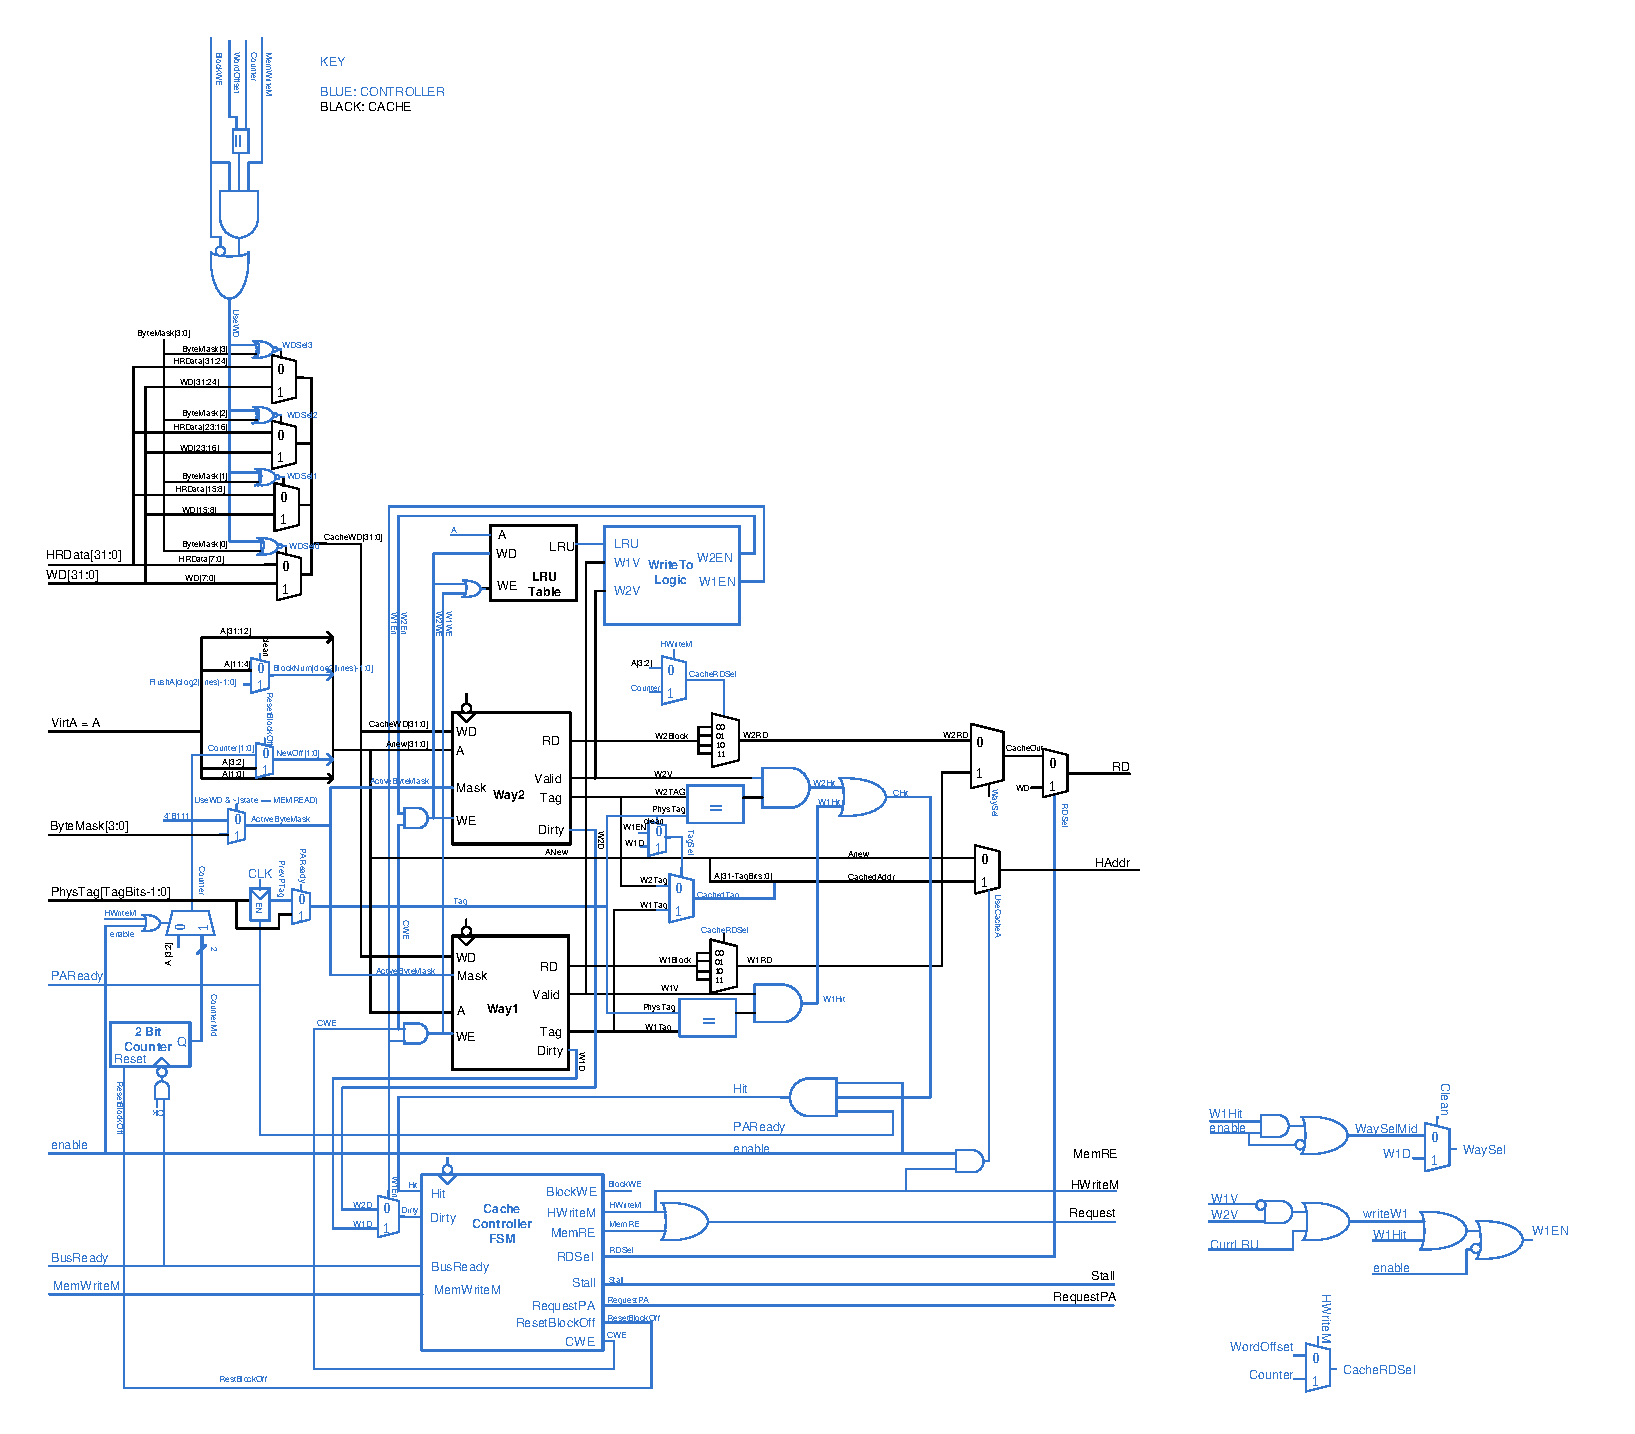
\includegraphics[width=\textwidth]{diagrams/dataCache.pdf}
	\caption{Diagram of 2 way set associative instruction cache. Controller logic in blue}
	\end{figure}

\subsection{All Relevant Files and Brief Descriptions}

	Table \ref{table:irel} shows the files that are used by the instruction cache and Table \ref{table:instrio} lists the top level inputs and outputs.

	\begin{table}
	\label{table:irel}
	\begin{tabular}{|l|p{70mm}|}
	\hline File  & Description \\ 
	\hline  instr\_cache.sv & Top level I\$ module \\ 
	\hline  instr\_cache\_controller.sv & Controller logic for the I\$.
	Contains the primary state machine described in section \ref{sec:istate} \\ 
	\hline  data\_writeback\_associative\_memory.sv & 
	Memory module containing the both cache ways, the LRU memory, and way selection mux's.
	This module is used in both the instruction and data caches.
	The instruction cache fixes the dirty and clean inputs to zero, because it is a read only cache.\\ 
	\hline  data\_writeback\_associative\_cache\_way.sv & 
	Contains the memory associated with one cache way. This includes four words per line along with the valid, and tag bits. \\ 
	\hline  word\_memory.sv & Byte addressable word memory  \\
	\hline
	\end{tabular} 
	\caption{Instruction cache files}
	\end{table}

	\begin{table}
	\label{table:instrio}
	\begin{tabular}{|l|p{85mm}|l|}
	\hline Port & Description & I/O \\ 
	\hline clk & Clock input &  I \\ 
	\hline reset & Global reset signal &  I \\ 
	\hline uOpStallD & Micro-Op stall signal. This signal is used to prevent repeated memory assesses when the pipeline is stalled &  I \\ 
	\hline A[31:0] & Virtual address from the leg datapath & I \\
	\hline CP15en & Enable signal from the coprocessor & I \\
	\hline AddrOp & Indicates coprocessor is invalidating using a virtual address instead of a set index. When high, only invalidate on a hit in the instruction cache.& I \\
	\hline InvAllMid & When InvAllMid and Inv are high, invalidate all lines from cache. This signal is driven by the coprocessor & I \\
	\hline Inv & Invalidate signal from the coprocessor & I \\
	% \hline CurrCBit & Cachable bit for the current TLB entry & I \\
	\hline PhysTag[tbits-1:0] & Physical Tag from the TLB & I \\
	\hline PAReadyF & Indicates TLB entry is valid for the instruction cache. The instruction cache uses the physical address and control bits from the TLB & I \\
	\hline FSel & Indicates instruction cache has control of the AHB Bus & I \\
	\hline BusReady & AHB Ready signal & I \\
	\hline HRData[31:0] & Data from the AHB Bus & I \\
	\hline RD[31:0] & Data output from the cache. This is the same as HWData. & O \\
	\hline IStall & IStall signal from the instruction cache controller & O \\
	\hline HRequestF & Request AHB control & O \\
	\hline HAddrF[31:0] & AHB address & O \\
	\hline RequestPA & Request a physical address from the TLB & O \\
	\hline
	\end{tabular} 
	\caption{Instruction cache I/O (instr\_cache.sv)}
	\end{table}
	% TODO: fix the label and reference

\subsection{Instruction Cache States}
\label{sec:istate}

Below is an explanation of the instruction cache states.

\begin{enumerate}
	\item READY 
	The ready state is the default state for the instruction cache.
	Upon a cache hit, the instruction cache will remain in the READY state.

	\item MEMREAD:
	Instruction cache enters this state on a cache miss to read data from memory.
	The cache reads four words sequentially from the AHB Bus.

	\item LASTREAD:
	The last memread state in the cache. 
	During this state, the instruction cache does not request a new memory access.
	It waits for the last memory read to complete.

	\item NEXTINSTR:
	The next instr state removes the stall on the pipeline and allows the instructions to move one stage down the pipeline. If this stage did not exist, then the instruction at the fetch stage would remain the same and after the requested instruction is retrieved, the same data would be retrieved again. 

\end{enumerate}
